\documentclass[]{rAMF2e}
%\usepackage[square]{natbib}
%\usepackage{authblk}
\usepackage{listings}
\usepackage[center]{caption}


\begin{document}
\doi{}
\issn{}  \issnp{}
\jvol{00} \jnum{00} \jyear{2013} %\jmonth{January--March}
\def\jobtag{}
\publisher{Unpublished}
\jname{}

\markboth{Fabien {Le Floc'h}, Gary Kennedy}{Draft}

\title{Finite Difference Techniques for Arbitrage Free SABR}
\author{Fabien {Le Floc'h}$^\star$\thanks{{\em{Correspondence Address}}: Calypso Technology, 106 rue de La Bo\'{e}tie, 75008 Paris. Email: \texttt{fabien\_lefloch@calypso.com} \vspace{6pt}} and Gary Kennedy$^\dag$}
\affil{$^\star$Calypso Technology, 106 rue de La Bo\'{e}tie, 75008 Paris\\$^\dag$Clarus Financial Technology, London}
%
\date{\today}
\received{v2.0 released August 2013}

\maketitle
\newcommand{\sgn}{\mathop{\mathrm{sgn}}}
\begin{abstract}
This paper presents various finite difference schemes applied to the SABR arbitrage free density problem with a focus on stability and speed.
\begin{keywords}stochastic volatility, SABR, TR-BDF2, Crank-Nicolson, finite difference, finance\end{keywords}
\end{abstract}

\section{Introduction}
It is now well known that original SABR analytic formula from \citep{hagan2002managing} used to compute option implied volatility is not arbitrage free as the probability density can become negative for low strikes and long maturities. Given the current low rates environment, many authors have proposed various improvements to the original formula \citep{obloj2008fine, johnson2009arbitrage, paulot2009asymptotic, benaim2008arbitrage}.  A single step finite difference method is proposed in \citep{andreasen2011zabr} which leads to an arbitrage free `SABR-like' model. Whilst the approach from Andreasen and Huge converges for short maturities to the original SABR analytic formula, it is (deliberately) different for longer expiries, even at the money.

Hagan recently proposed a new arbitrage free SABR solution, based on a finite difference discretisation of the probability density in \citep{hagan2013arbitrage}. This approach provides a solution very close to the original SABR analytic formula, well known and widely used, while being arbitrage free, and thus allowing pricing with low rates. The authors use a Crank-Nicolson time-stepping scheme, which is known to have oscillation issues \citep{duffy2004critique,GiCa2006} as it is only $A$-stable but not $L$-stable \citep{Le07}. We will show that this issue arises in the context of SABR pricing, and propose alternative schemes that are not very well known in computational finance, and yet are effective on this problem. One such scheme is TR-BDF2, used in the semiconductor industry as well as more generally in computational physics \citep{bank1985transient,bathe2005composite,edwards2011nonlinear, flavell2013conservative}. Another scheme is due to Lawson and Swayne; whilst somewhat obscure, it is simple and effective on this problem \citep{lawson1976simple}.  

Speed and accuracy were key ingredients in popularising the original SABR formula. Given that for a 30 year cap on a 3M LIBOR, there are potentially 119 PDEs to solve, we will focus our attention on the performance of the proposed schemes, as well as to what extent the discretisation grid can be reduced in size.



\section{Arbitrage Free SABR}
In \citep{hagan2013arbitrage}, pricing with SABR parameters $\alpha, \beta, \rho, \nu$ and forward $f$ at $\tau_{ex}$ relies on the solution of a PDE on the probability density $Q$:

\begin{align}\label{eqn_pde}
\frac{\partial Q}{\partial T}(T,F) = \frac{\partial^2 M(T,F) Q(T,F)}{\partial F^2} \text{ and } \begin{cases}
\frac{\partial Q_L}{\partial T}(T) = \lim_{F \to F_{min}} \frac{\partial M(T,F) Q(T,F)}{\partial F}\\
\frac{\partial Q_R}{\partial T}(T) = \lim_{F \to F_{max}} \frac{\partial M(T,F) Q(T,F)}{\partial F}
\end{cases}
\end{align}
with
\begin{alignat}{2}
M(T,F) = \frac{1}{2} D^2(F) E(T,F) \text{, } E(T,F) = e^{\rho\nu\alpha\Gamma(F) T} \text{, } \Gamma(F) = \frac{F^{\beta}-f^{\beta}}{F-f}\\
D(F) = \sqrt{\alpha^2 +2\alpha\rho\nu y(F)+ \nu^2 y(F)^2} F^{\beta} \text{, } y(F) = \frac{F^{1-\beta}-f^{1-\beta}}{1-\beta}
\end{alignat}

It is suggested that the lower boundary $F_{min}$ for the standard SABR model is placed at or near zero. However, the finite difference grid described in Appendix C of their paper starts at  $F_0 = F_{min} - \frac{h}{2}$, where, $h$ is the asset forward discretisation step size, potentially requiring the evaluation of functions not well-defined for negative values of $F_0$. Fortunately, only the product $M_0 Q_0$ is used in the discretisation of equation (\ref{eqn_pde}) and it is entirely defined by $M_1 Q_1$  because of the mirror-like boundary condition (imposed at the fictitious point $F_0$): 
\begin{align}\label{boundary_condition}
M_0 Q_0 + M_1 Q_1 &= 0
\end{align}
As long as $M_0 \neq 0$, $M_0 Q_0$ will take the value $-M_1 Q_1$. For example, we can use $|F_0|$ to compute $M_0$ and this will result in a symmetry around $F_{min}$.


Another alternative would be to place the grid so that $F_0 = F_{min}$ and use boundary condition $Q_0 = 0$ there. The probability of absorption $Q_L$ could then be evaluated using an forward finite difference first derivative estimate. This would result in the exact same equation as (C.10a) of their paper and the scheme would still be moment preserving. However this comes at a cost of a slight loss of accuracy as, effectively, the derivative will be estimated using $Q_1 = Q(h)$ instead of $Q_1 = Q(\frac{h}{2})$.

The formula for $\Gamma$ is also undefined for $F=f$, in which case we just use $\Gamma(f) = \frac{\partial C}{\partial F}(f)$.

\section{Change of Variable}
One practical difficulty that arises with the Arbitrage Free PDE described in equations (\ref{eqn_pde}) is the choice of $F_{max}$. \citet{hagan2013arbitrage} proposes a formula to estimate the required $F_{max}$, that, for some parameters is not suitable. It can be very large for long term deals and as a consequence the discretization requires a very large number of points to obtain an acceptable accuracy. The technique becomes inefficient. A change of variable is proposed in \citep{hagan2013change} as a remedy:
\begin{align}
z(F) &= \int_{f}^F \frac{dF'}{D(F')}
\end{align}
This leads to a PDE in $\theta(z) = Q(T,F(z))D(F(z)) = Q(T,F(z))C(z)$ with $C(z) = D(F(z))$:
\begin{align}\label{eqn-transform-pde}
\frac{\partial \theta}{\partial T}(T,z) = \frac{1}{2} \frac{\partial}{\partial z} \left\lbrace \frac{1}{C(z)} \frac{\partial C(z)E(T,z)\theta(T,z)}{\partial z} \right\rbrace
 \text{ and } \begin{cases}
\theta(T,z) = 0 \text{ as } z \to z^{-}=z(F_{min})\\
\theta(T,z) = 0 \text{ as } z \to z^{+}=z(F_{max})
\end{cases}
\end{align}
with \begin{align}
y(z) &= \frac{\alpha}{\nu}\left[ \sinh(\nu z) + \rho (\cosh(\nu z) - 1) \right]\\
F(y) &= \left[ f^{1-\beta} + (1-\beta)y \right]^{\frac{1}{1-\beta}}
\end{align}

The probability at the boundaries accumulates according to:
\begin{align}\label{eqn-transform-boundary}
\frac{\partial P_L}{\partial T}(T) &= \lim_{z \to z^{-}} \frac{1}{2} \frac{1}{C(z)} \frac{\partial C(z)E(T,z)\theta(T,z)}{\partial z}\\
\frac{\partial P_R}{\partial T}(T) &= \lim_{z \to z^{+}}  -\frac{1}{2} \frac{1}{C(z)} \frac{\partial C(z)E(T,z)\theta(T,z)}{\partial z}
\end{align}

As a result, the effect of the diffusion term $D$ has almost been cancelled, and the probability density $\theta$ is closer to a Gaussian in $z$. $z^+$ and $z^-$ are then naturally chosen to be $\pm n_{sd}\sqrt{T}$, corresponding to $n_{sd}$ standard deviations above and below the forward located at $z=0$ (taking care of truncating at the barrier $F=0$ if necessary). Figure \ref{fig:Fz} shows that the probability density will be computed with a high concentration of points around the forward, and a much lower one near the upper boundary.

\begin{figure}[htb]
  \begin{center}  
    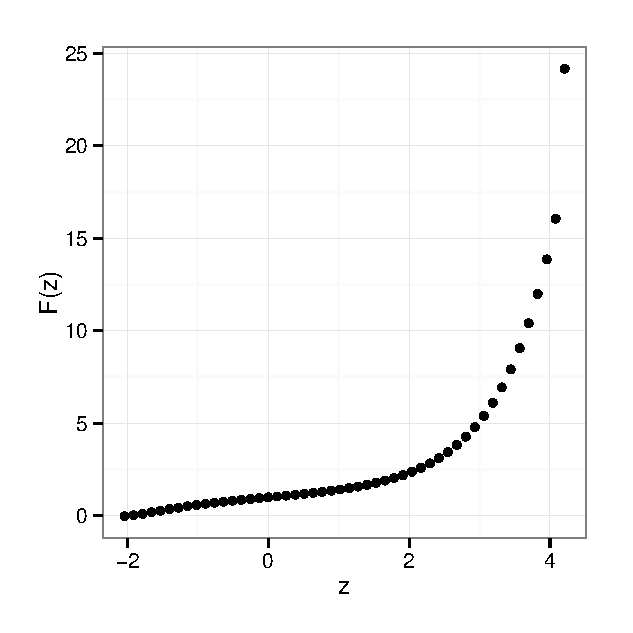
\includegraphics[width=6cm]{fz.eps}
  \end{center}
     \caption{\label{fig:Fz} F(z) with $\alpha=35\%, \beta=0.25, \rho=-10\%, \nu=100\%, \tau_{ex}=1$}
\end{figure}

For some extreme SABR parameters, the change of variable allows high accuracy with a small number of points. The uniform discretization of $Q$ in $F$ can require approximately 1000 times more points to reach a similar accuracy (Table \ref{table:discretization}).
\begin{table}[h]
\begin{center}
\begin{tabular}{|c|r|r|r|r|}
\hline
\multicolumn{5}{|c|}{Uniform discretization of $Q$ in $F$} \\ \hline
$F_{max}$ & Points & Steps & Price & Vol \\
5 & 100 & 10 & 0.64082 & 85.118  \\
50 & 100 & 10 & 0.78764 & 155.683\\
500 & 1000 & 10 & 0.79780 & 191.493 \\
5000 & 10000 & 160 & 0.79835 & 196.926\\
\hline
\end{tabular}
\begin{tabular}{|c|r|r|r|r|}
\hline
\multicolumn{5}{|c|}{Discretization of $\theta$ in $z$} \\ \hline
$n_{sd}$ & Points & Steps & Price & Vol\\
3 & 10 & 10 & 0.79819 & 195.243\\
3 & 100 & 10 & 0.79845 & 198.135\\
4 & 100 & 10 & 0.79845 & 198.130\\
10 & 10000 & 160 & 0.79845 & 198.130\\
\hline
\end{tabular}
\caption{\label{table:discretization}Price by TR-BDF3 without and with variable change for extreme SABR parameters: $\alpha=100\%, \beta=0.30, \rho=90\%, \nu=100\%, \tau_{ex}=10, f=1$}
\end{center}
\end{table} 
The number of points used can not be too small: the forward should not be on the boundary. This restriction is much stricter for the uniform discretization of $Q$ than for the discretization in the changed variable $\theta$.

\section{Crank-Nicolson Oscillations with SABR}\label{section_cn}
\begin{figure}[htb]
  \begin{center}  
    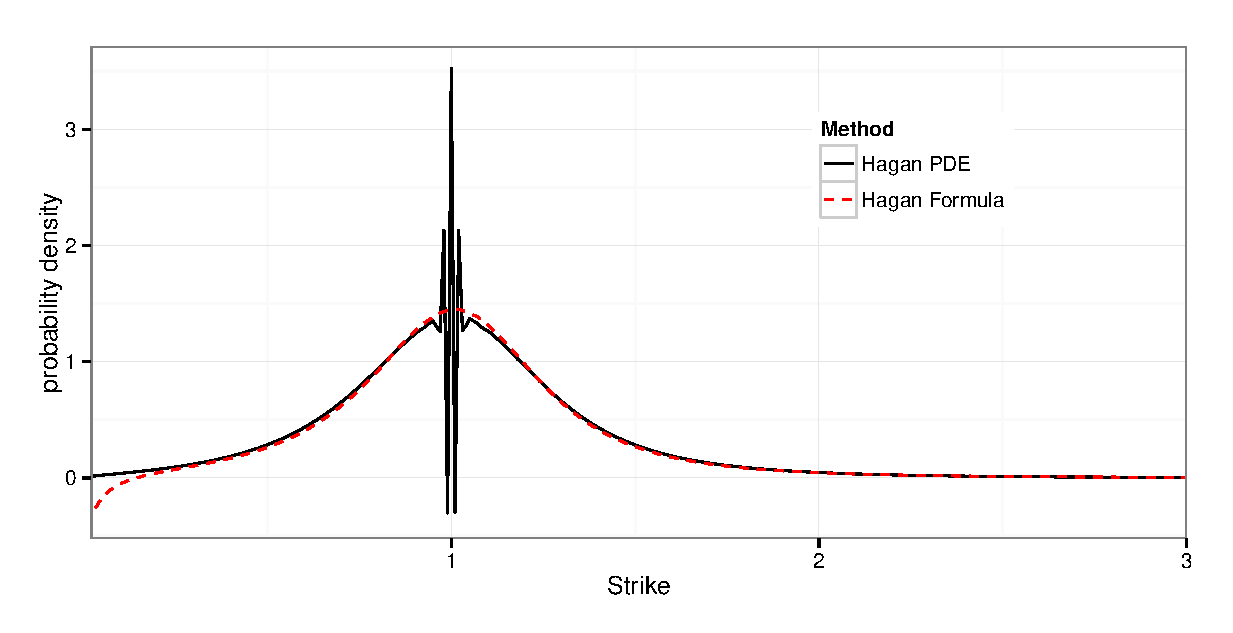
\includegraphics[width=12cm]{density_hagan_cn_500_40.eps}
  \end{center}
     \caption{\label{fig:density_hagan_cn_500_40} Probability density in Hagan PDE discretised with Crank-Nicolson with 500 points and 40 time-steps. $\alpha=35\%, \beta=0.25, \rho=-10\%, \nu=100\%, \tau_{ex}=1$}
\end{figure}

We use the same parameters as the example of negative density with the standard SABR formula in \citep{hagan2013arbitrage}: $\alpha=35\%, \beta=0.25, \rho=-10\%, \nu=100\%$ and forward $f=1$ at $\tau_{ex}=1$, a relatively fine discretisation in the rate dimension (500 points, that is $h = 0.01005$) and large time-steps (40 steps, that is $\delta=0.025$). \cite{hagan2013arbitrage} recommend between 200 and 500 points and 30 to 100 time-steps.

Figure \ref{fig:density_hagan_cn_500_40} shows strong oscillations around the forward. To guarantee the absence of oscillations, the \emph{Courant number}  should be small enough $\Psi \leq 1$ (Theorem 2.2 in \cite{morton2005numerical}). For the uniform discretization of $Q(F)$, $\Psi_Q = M \frac{\delta}{h^2}$. This corresponds directly to the stability of the explicit Euler part of Crank-Nicolson. In practice, a higher value is acceptable because of a slight damping in Crank-Nicolson \citep{lawson1978extrapolation}. Although $M$ depends on $F$, we can use the at-the-money value at $f$, as the spike is located there; that is, 
\begin{align}
\Psi_Q &= \frac{1}{2} \alpha^2 f^{2\beta} \frac{\delta}{h^2} \\
\Psi_{\theta} &= f^{\beta}\frac{\delta}{h^2} 
\end{align} 

\begin{figure}[htb]
  \begin{center}  
    \subfigure[with 40 time steps $\Psi_Q = 15.16$]{\label{fig:density_hagan_cn_500_40_5}
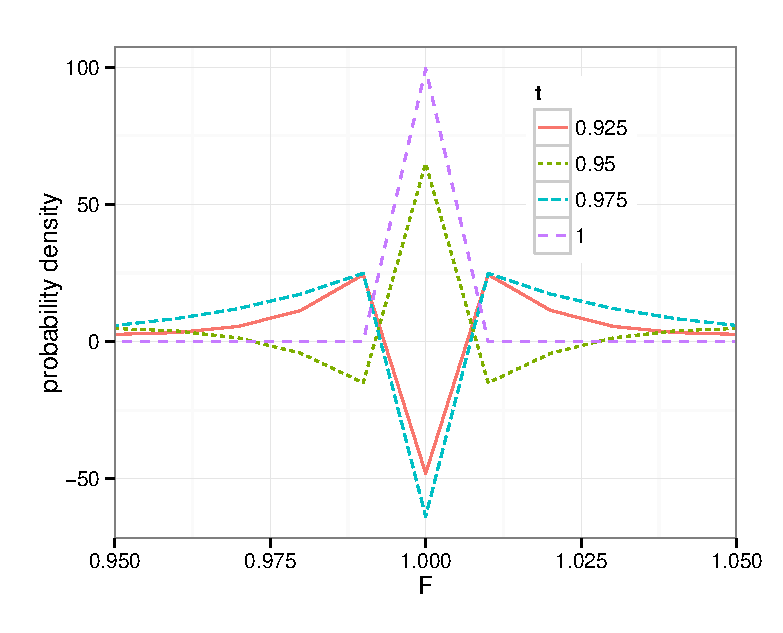
\includegraphics[width=7cm]{density_hagan_cn_500_40_5.eps}}
  \subfigure[with 1280 time steps $\Psi_Q = 0.47$]{\label{fig:density_hagan_cn_500_1280_5}
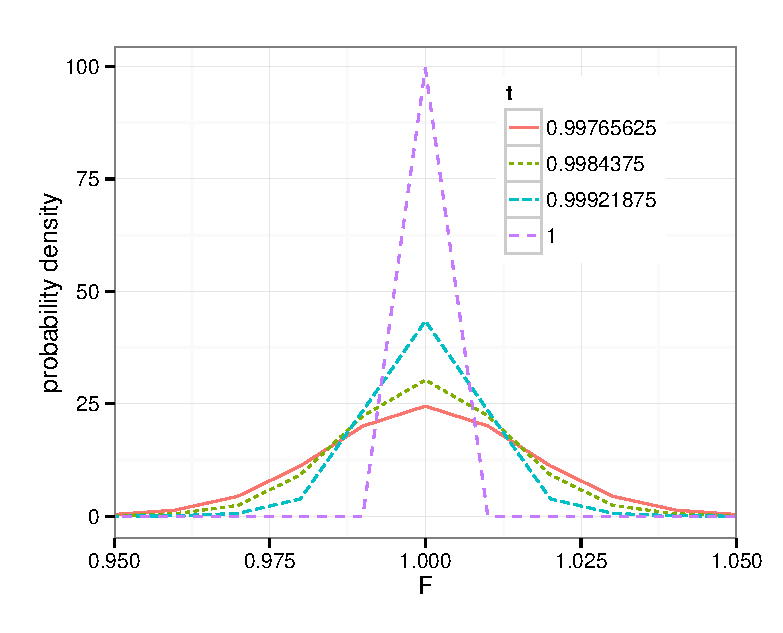
\includegraphics[width=7cm]{density_hagan_cn_500_1280_5.eps}}
  \end{center}
     \caption{\label{fig:density_hagan_500_40_5} First 4 time steps of the probability density in Hagan PDE discretised with Crank-Nicolson}
\end{figure}

In our example, in Figures \ref{fig:density_hagan_cn_500_40} and \ref{fig:density_hagan_cn_500_40_5} $\Psi_Q \approx 15$ while Figure \ref{fig:density_hagan_cn_500_1280_5} shows that indeed when $\Psi < 1$ there are no oscillations. The Crank-Nicolson oscillations are even stronger with the PDE in $\theta$ as for $\alpha \ll 1$, we have $\Psi_{\theta} \gg \Psi_Q$. Using the same SABR parameters and $n_{sd}=3$ (corresponding to $F_{max} \approx 5$), $\Psi_{\theta} \approx 250$. In the next sections it is shown that a much smaller number of time steps can be used with other finite difference time-stepping techniques whilst still preserving good accuracy.

\section{Alternative Schemes}
The boundary condition described by equation (\ref{boundary_condition}) is applicable to all schemes considered in this section as it is independent of the time-stepping.

\subsection{Rannacher}
A common fix for Crank-Nicolson oscillations related to non smooth initial data is Rannacher time-stepping \citep{rannacher1984finite, GiCa2006}. It consists of introducing two half time-steps of implicit Euler time-stepping before applying Crank-Nicolson, because implicit Euler has much stronger damping properties. This comes at a cost in accuracy as implicit Euler is an order-1 scheme in time, especially when only a few time-steps are needed. 
The SABR density discretisation will still be moment preserving if we discretise the Euler half steps as:
\begin{align}\label{eqn_euler_1}
Q_j^{n+\frac{1}{2}}-Q_j^n &= \frac{\delta}{2h^2} \left(M_{j+1}^{n+\frac{1}{2}}Q_{j+1}^{n+\frac{1}{2}}-2M_j^{n+\frac{1}{2}}Q_j^{n+\frac{1}{2}}+M_{j-1}^{n+\frac{1}{2}}Q_{j-1}^{n+\frac{1}{2}} \right) \\
\label{eqn_euler_2}
Q_L^{n+\frac{1}{2}}-Q_L^n &= \frac{\delta}{2h} \left(M_{1}^{n+\frac{1}{2}}Q_{1}^{n+\frac{1}{2}}-M_0^{n+\frac{1}{2}}Q_0^{n+\frac{1}{2}}\right) \\
Q_R^{n+\frac{1}{2}}-Q_R^n &= -\frac{\delta}{2h} \left(M_{J+1}^{n+\frac{1}{2}}Q_{J+1}^{n+\frac{1}{2}}-M_J^{n+\frac{1}{2}}Q_J^{n+\frac{1}{2}}\right) 
\end{align}
for $j=1,...,J$ and $n=0,\frac{1}{2}, 1, \frac{3}{2}$.

\subsection{Implicit Richardson Extrapolation}
A simple Richardson extrapolation in time \citep{richardson1911approximate} on implicit Euler will also provide a nearly order-2 scheme in time, keeping strong damping properties of the implicit Euler scheme at the cost of increased computational load: the implicit Euler scheme (Equations \ref{eqn_euler_1}, \ref{eqn_euler_2}) is evaluated with $\frac{\delta}{2}$ and $\delta$. In practice it is around twice as slow as Crank-Nicolson. At $T=N\delta=\tau_{ex}$, we apply:
\begin{align}\label{eqn_richardson}
Q(F) &= 2 \hat{Q}^{\frac{\delta}{2}}(F) - \hat{Q}^{\delta}(F) \\
Q_L &= 2 \hat{Q}^{\frac{\delta}{2}}_L - \hat{Q}^{\delta}_L\\
Q_R &= 2 \hat{Q}^{\frac{\delta}{2}}_R - \hat{Q}^{\delta}_R
\end{align}

where $\hat{Q}^{\delta}$ is $Q$ computed by implicit Euler with a time step of $\delta$.


\subsection{Lawson-Morris-Gourlay}
A local Richardson extrapolation in time of second and third order is proposed in \citep{lawson1978extrapolation} and \citep{gourlay1980extrapolation}. In practice, it is a faster alternative to the standard Richardson extrapolation because the tridiagonal matrix stemming out of the finite difference discretisation can be reused, while keeping $L$-stability and thus strong damping properties.

For the second order scheme, at each time-step, equation (\ref{eqn_richardson}) is applied.
For the third order scheme, at each time-step we apply:
%\begin{subequations}
\begin{align}\label{eqn_lmg3}
Q(F) &= 4.5 \hat{Q}^{\frac{\delta}{3}}(F) - 4.5 \hat{Q}^{\frac{2\delta}{3}}(F)  + \hat{Q}^{\delta}(F)\\
Q_L &= 4.5 \hat{Q}^{\frac{\delta}{3}}_L - 4.5 \hat{Q}^{\frac{2\delta}{3}}_L  + \hat{Q}^{\delta}_L\\
Q_R &= 4.5 \hat{Q}^{\frac{\delta}{3}}_R - 4.5 \hat{Q}^{\frac{2\delta}{3}}_R  + \hat{Q}^{\delta}_R
\end{align}
%\end{subequations}
where $\hat{Q}^{\frac{\delta}{3}}$ is $Q$ computed by implicit Euler with 3 time steps of $\frac{\delta}{3}$ and $\hat{Q}^{\frac{2\delta}{3}}$ is $Q$ computed by implicit Euler with a time step of $\frac{2\delta}{3}$ and $\frac{\delta}{3}$. Being linear combinations of implicit Euler, those schemes are moment preserving.

\subsection{Lawson-Swayne}
A slightly faster second order unconditionally stable scheme is presented as a remedy to Crank-Nicolson in \citep{lawson1976simple, lawson1978extrapolation}. Let $b=1-\frac{\sqrt{2}}{2}$, it consists in applying two implicit Euler steps with time-step of $b\delta$ and an extrapolation on the values at those two steps.\\
\\
First stage:
\begin{subequations}
\begin{align}\label{eqn_lawson_swayne}
\begin{split}
Q_j^{n+b}-Q_j^n &= \frac{b\delta}{h^2} \left(M_{j+1}^{n+b}Q_{j+1}^{n+b}-2M_j^{n+b}Q_j^{n+b}+M_{j-1}^{n+b}Q_{j-1}^{n+b} \right) \\
Q_L^{n+b}-Q_L^n &= \frac{b\delta}{h} \left(M_{1}^{n+b}Q_{1}^{n+b}-M_0^{n+b}Q_0^{n+b}\right) \\
Q_R^{n+b}-Q_R^n &= -\frac{b\delta}{h} \left(M_{J+1}^{n+b}Q_{J+1}^{n+b}-M_J^{n+b}Q_J^{n+b}\right)
\end{split}\\
\intertext{Second stage:}
\begin{split}
Q_j^{n+2b}-Q_j^{n+b} &= \frac{b\delta}{h^2} \left(M_{j+1}^{n+2b}Q_{j+1}^{n+2b}-2M_j^{n+2b}Q_j^{n+2b}+M_{j-1}^{n+2b}Q_{j-1}^{n+2b} \right) \\
Q_L^{n+2b}-Q_L^{n+b} &= \frac{b\delta}{h} \left(M_{1}^{n+2b}Q_{1}^{n+2b}-M_0^{n+2b}Q_0^{n+2b}\right) \\
Q_R^{n+2b}-Q_R^{n+b} &= -\frac{b\delta}{h} \left(M_{J+1}^{n+2b}Q_{J+1}^{n+2b}-M_J^{n+2b}Q_J^{n+2b}\right)
\end{split}\\
\intertext{And finally:}
\begin{split}
Q_j^{n+1} &= (\sqrt{2}+1) Q_j^{n+2b} - \sqrt{2}Q_j^{n+b}\\
Q_L^{n+1} &= (\sqrt{2}+1) Q_L^{n+2b} - \sqrt{2} Q_L^{n+b}\\
Q_R^{n+1} &= (\sqrt{2}+1)  Q_R^{n+2b} - \sqrt{2} Q_R^{n+b}
\end{split}
\end{align}
\end{subequations}
for $j=1,...,J$ and $n=0,...,N-1$.

The scheme is moment preserving as it can also be seen as a linear combination of implicit Euler schemes.

\subsection{TR-BDF2}
TR-BDF2 is a two-stage method where the first stage consists in applying the (weighted) trapezoidal rule (Crank-Nicolson) and the second stage consists in applying the second order backward difference scheme (BDF2) on the first stage result and the first stage initial input \citep{bank1985transient, Le07}. It is second order accurate in time and $L$-stable. It is not to be confused with the simpler multistep method BDF2: the full step only depends on the previous full step while BDF2 depends on the two previous timesteps and can lose its accuracy \citep{windcliff2001shout} with variable timesteps and linear complimentary problems. This scheme does not suffer from such drawbacks. The scheme has been applied to finance in the context of American option pricing \citep{floc2013tr}.
\begin{subequations}
\begin{align}
Q^{n+\alpha} &= Q^n + \frac{\alpha \delta}{2}\left(\frac{\partial^2 M^{n} Q^n}{\partial F^2}+\frac{\partial^2 M^{n+\alpha} Q^{n+\alpha}}{\partial F^2}\right)\\
Q^{n+1} &= \frac{1}{2-\alpha}\left(\frac{1}{\alpha} Q^{n+\alpha} - \frac{(1-\alpha)^2}{\alpha}Q^n + \delta(1-\alpha)\frac{\partial^2 M^{n+1} Q^{n+1}}{\partial F^2}\right)
\end{align}
\end{subequations}

The weight $\alpha$ can be chosen to match Crank-Nicolson ($\alpha=\frac{1}{2}$) or to have proportional Jacobians ($\alpha = 2-\sqrt{2}$). The later provides optimal stability \citep{dharmaraja2009optimal}. 

This can be extended to three-stages, with two stages of the trapezoidal rule and one stage of third order backward difference scheme (BDF3) as in \citep{bathe2005composite}, resulting in a method with even stronger damping properties:
\begin{subequations}
\begin{align}
Q^{n+\frac{1}{3}} &= Q^n + \frac{\delta}{6}\left(\frac{\partial^2 M^{n} Q^n}{\partial F^2}+\frac{\partial^2 M^{n+\frac{1}{3}} Q^{n+\frac{1}{3}}}{\partial F^2}\right)\\
Q^{n+\frac{2}{3}} &= Q^n + \frac{\delta}{6}\left(\frac{\partial^2 M^{n+\frac{1}{3}} Q^{n+\frac{1}{3}}}{\partial F^2}+\frac{\partial^2 M^{n+\frac{2}{3}} Q^{n+\frac{2}{3}}}{\partial F^2}\right)\\
Q^{n+1} &= \frac{1}{11}\left( 18 Q^{n+\frac{2}{3}} - 9Q^{n+\frac{1}{3}} + 2Q^n + 2\delta\frac{\partial^2 M^{n+1} Q^{n+1}}{\partial F^2}\right)
\end{align}
\end{subequations}

\subsection{Smoothing before Crank-Nicolson}
Similarly to Rannacher idea, we could use Lawson-Morris-Gourlay for the first few timesteps in order to dampen the oscillations before applying Crank-Nicolson. This ensures an overall order-2 accuracy, even with a low number of time-steps. TR-BDF2 and TR-BDF3 fit particularly well as the first stages are a weighted Crank-Nicolson. So one could stop doing the BDF2 (respectively BDF3) stages when the solution is sufficiently smooth. 

We found by experimentation that Crank-Nicolson, dampened by 4 initial steps of TR-BDF2 or Lawson-Swayne was very efficient, but we are less comfortable recommending such a hybrid scheme without further analysis.

\subsection{Optimising for Performance}
The function $M(F,T)$ needs to be computed for every grid point $\left(F_j, t_n\right)$. The performance of the overall algorithm can be greatly improved by minimising the calls to the \texttt{pow} and \texttt{exp} functions as those are expensive. The quantities $\frac{1}{2} \alpha^2 (1+2\rho\nu z+ \nu^2 z^2) C^2(F)$ and $\rho\nu\alpha\Gamma$ are constant in time and can be thus be cached between time-steps. A further improvement is to decompose $t_{n+1}$ as $t_{n}+\delta$, then 
\begin{equation}
e^{\rho\nu\alpha\Gamma t_{n+1}}=e^{\rho\nu\alpha\Gamma t_n}e^{\rho\nu\alpha\Gamma \delta}
\end{equation}
We can therefore just compute the initial value $\frac{1}{2} \alpha^2 (1+2\rho\nu z+ \nu^2 z^2) C^2(F)$ together with $e_j = e^{\rho\nu\alpha\Gamma(F_j) \delta}$ for $j=0,...,J+1$ once, and at each step simply update $M$ as:
\begin{equation}
M_j^{n+1} = e_j M_j^{n} 
\end{equation}
This can be easily extended to multiple time-step sizes used in multi-stage schemes.

For multi-stage schemes, it is also possible to consider $M$ as piecewise constant between full time-steps and thus to avoid its computation for fractions of time-steps. In our tests, this led to a slightly decreased accuracy and little performance gain. The increase in error was particularly visible for long term options and large time-steps. We did not make that approximation for the tests presented in the next section.

\section{Numerical Results}
\subsection{Oscillations}
\begin{figure}[htb]
  \begin{center}  
  \subfigure[$t_N=T$]{\label{fig:density_hagan_ran_500_5_0}
  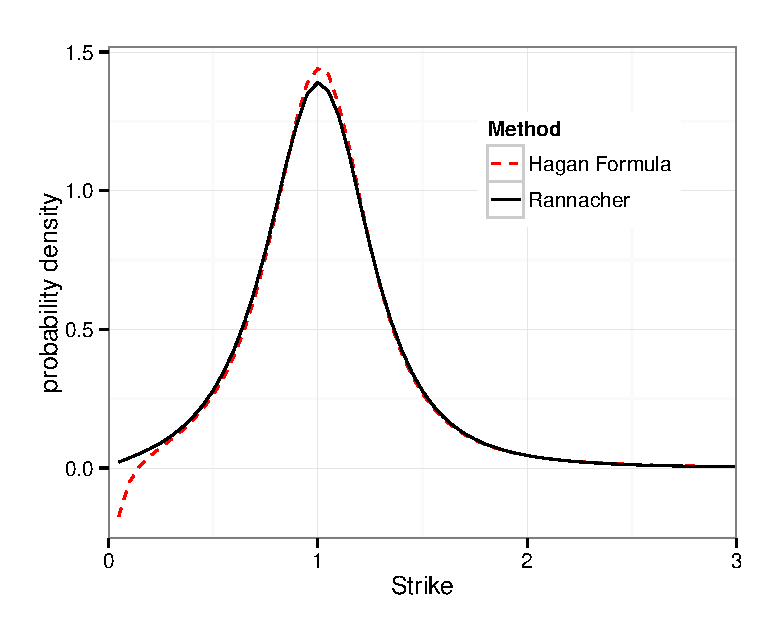
\includegraphics[width=7cm]{density_hagan_ran_500_5.eps}}
  \subfigure[Crank-Nicolson first 4 time steps with 5 time steps]{\label{fig:density_hagan_cn_500_5_5}
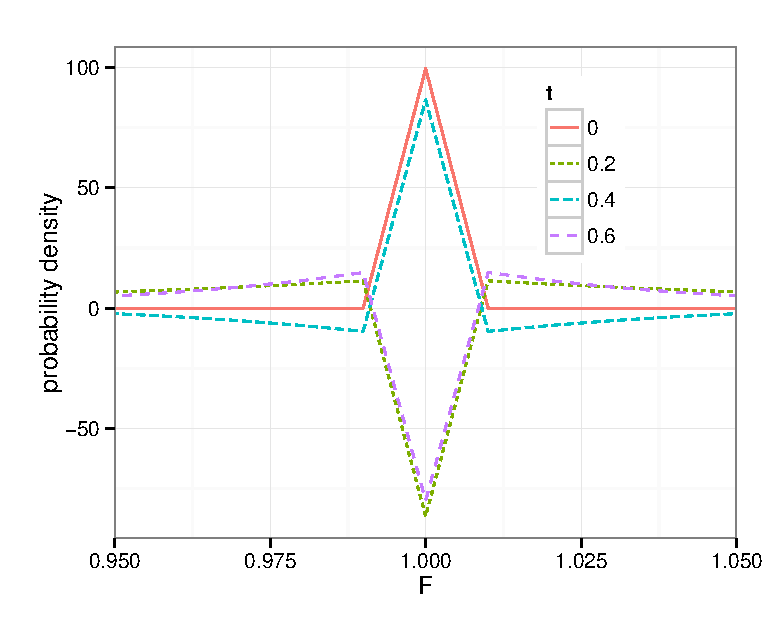
\includegraphics[width=7cm]{density_hagan_cn_500_5_5.eps}}
  \subfigure[Rannacher first 4 time steps with 5 time steps]{\label{fig:density_hagan_ran_500_5_5}
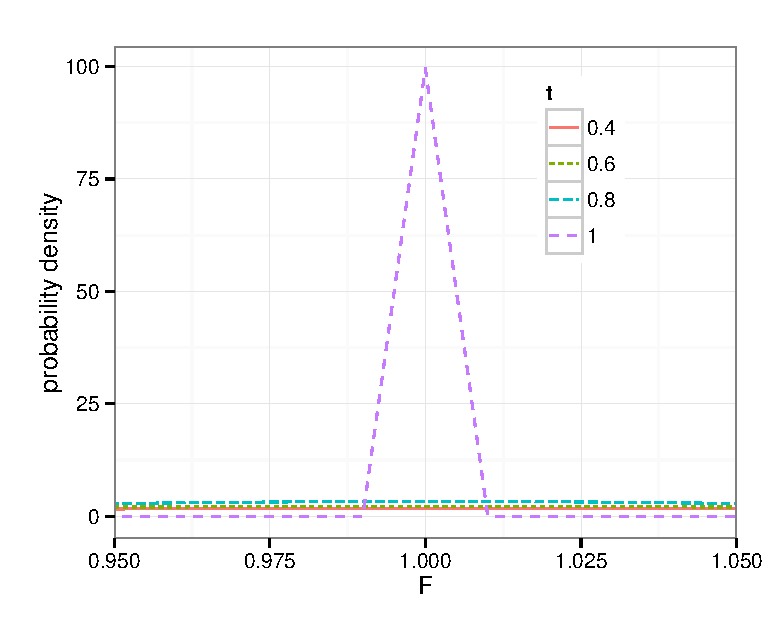
\includegraphics[width=7cm]{density_hagan_ran_500_5_5.eps}}
  \subfigure[LMG3 first 4 time steps with 5 time steps]{\label{fig:density_hagan_lmg3_500_5_5}
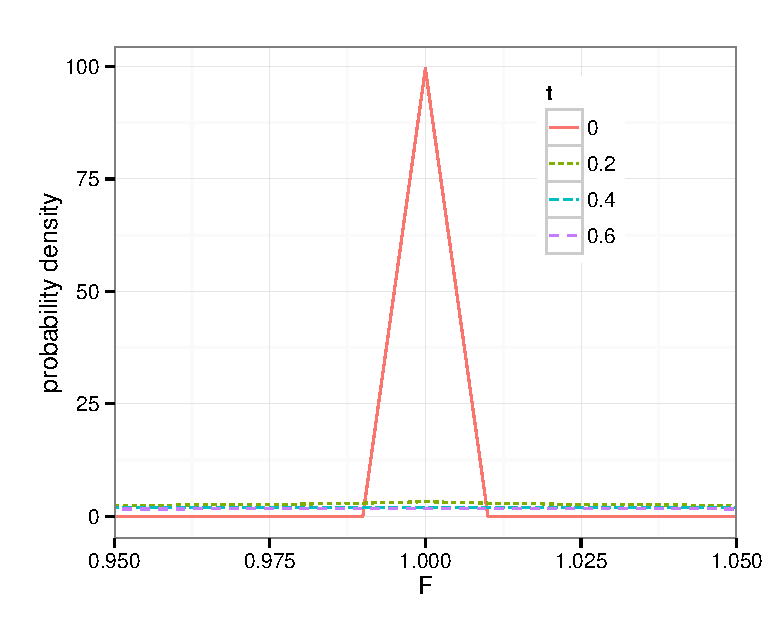
\includegraphics[width=7cm]{density_hagan_lmg3_500_5_5.eps}}
  \end{center}
     \caption{\label{fig:density_hagan_lmg2_500_10} Probability density in Hagan PDE using a total of 5 time-steps}
\end{figure}
With the same parameters as in section \ref{section_cn}, Figure \ref{fig:density_hagan_ran_500_5_0} shows a smooth positive probability density using only a total of 5 time-steps when Rannacher smoothing is applied to Crank-Nicolson. The density computed using second or third order Lawson-Morris-Gourlay (LMG2, LMG3), Lawson-Swayne (LS), TR-BDF2 or Richardson extrapolation on implicit Euler would look very similar. Figures \ref{fig:density_hagan_ran_500_5_5} and \ref{fig:density_hagan_lmg3_500_5_5} show no apparent oscillations in the first steps.
In contrast, Crank-Nicolson had strong oscillations visible at $T=\tau_{ex}$ with 40 time steps.

\subsection{Performance}
\subsubsection{Hagan Example}
With the same parameters as in section \ref{section_cn}, we look at the maximum error in the probability density with a varying number of time-steps compared to a Crank-Nicolson scheme with 5120 points for the rate dimension and 81920 time-steps. 

\begin{figure}[htb]
  \begin{center}  
  \subfigure[Accuracy vs. number of time steps]{\label{fig:perf_hagan_500_steps}
  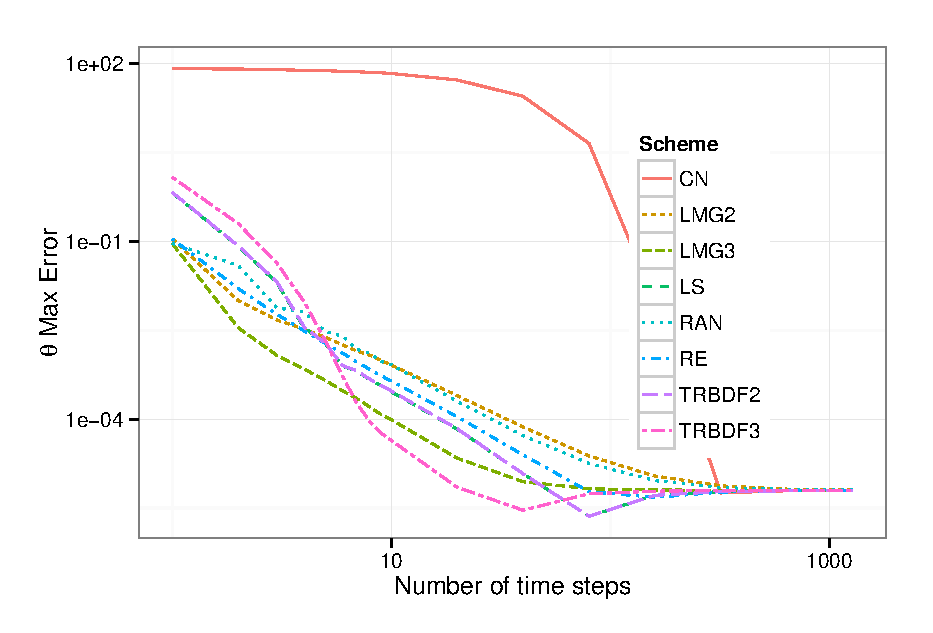
\includegraphics[width=7cm]{perf_theta_hagan_500_steps.eps}}
  \subfigure[Accuracy vs. time]{
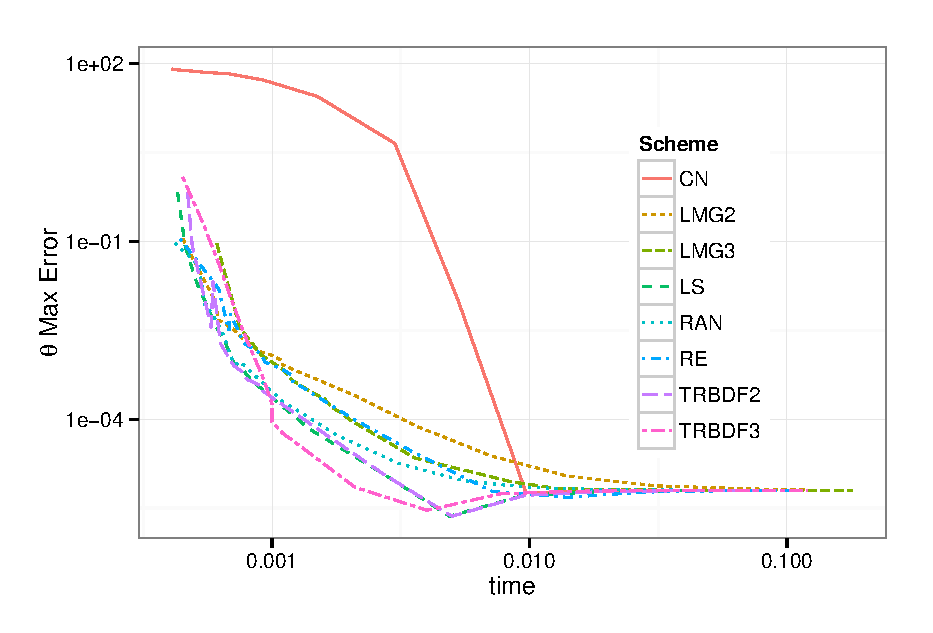
\includegraphics[width=7cm]{perf_theta_hagan_500_time.eps}}
    \end{center}
     \caption{\label{fig:perf_hagan_500} Performance on Hagan example}
\end{figure}

%show convergence graph
Other tests we performed indicate that the implied volatility maximum error or even the at-the-money implied volatility error would lead to similar conclusions. Furthermore, a Black implied volatility with an absolute error under 0.1\% was achieved with only 2 time steps for LMG3, Lawson-Swayne and TR-BDF2, 5 time steps for LMG2, and 10 steps for RAN. Lawson-Swayne is the most efficient scheme on this problem, closely followed by TR-BDF2, Rannacher and LMG3.

\subsubsection{Andreasen-Huge Example}
We consider the SABR parameters used in \citep{andreasen2011zabr}: $\alpha=0.0873, \beta=0.7, \rho=-0.48, \nu=0.47$ with a forward of $f=0.025$ and a maturity $\tau_{ex}=10.0$ and look at the maximum error in implied volatility between $0.2f$ and $2f$.

\begin{figure}[htb]
  \begin{center}  
  \subfigure[Accuracy vs. number of time steps]{\label{fig:perf_ah_500_steps}
  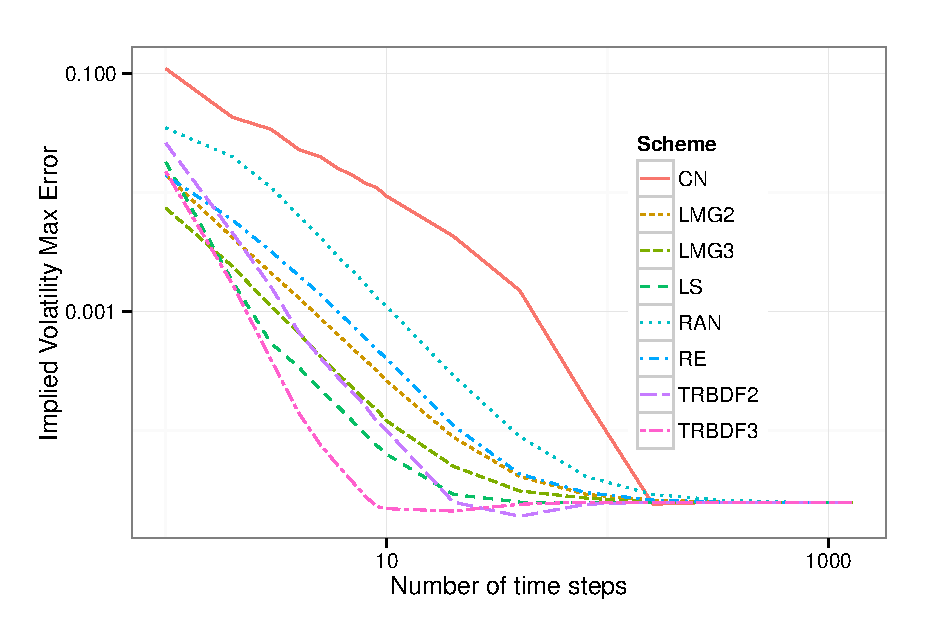
\includegraphics[width=7cm]{perf_vol_theta_ah_500_steps.eps}}
  \subfigure[Accuracy vs. time]{
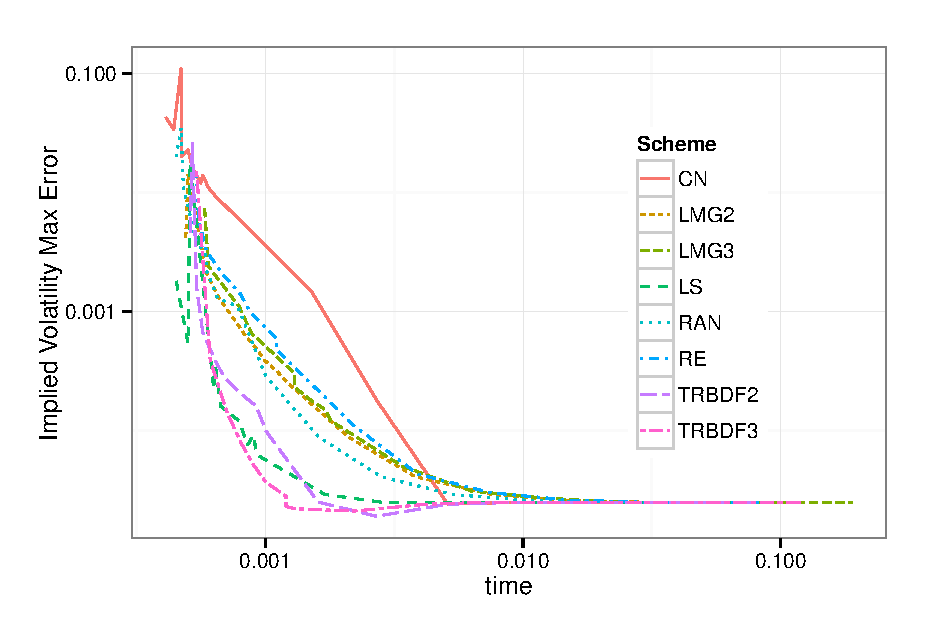
\includegraphics[width=7cm]{perf_vol_theta_ah_500_time.eps}}
    \end{center}
     \caption{\label{fig:perf_ah_500} Performance on Andreasen-Huge example}
\end{figure}


%show convergence graph

Only 2 time-steps are enough with  LMG3 for good accuracy, and 5 for LMG2, LS, RAN and TR-BDF2. 

\section{Conclusion}
It is possible to accurately compute option prices under the arbitrage free SABR approach with very few time-steps, even for long maturities. The Rannacher smoothing is a particularly simple and efficient way to improve accuracy significantly compared to Crank-Nicolson on this problem. Other schemes such as TR-BDF2 or Lawson-Swayne can be even more efficient. In our experiments TR-BDF2 and Lawson-Swayne were robust and had similar stability and convergence properties.


Thus, with a careful choice of finite difference scheme, \citep{hagan2013arbitrage} is particularly competitive to the one step finite difference approach of \citep{andreasen2011zabr}.

\bibliographystyle{rAMF}
%\bibliographystyle{ieeetr}
\bibliography{lefloch_sabr_fdm}
\newpage

\section{Example Code}
For illustration purpose, we detail here Octave code (also working with Matlab) for pricing vanilla options under the Arbitrage Free SABR model using Lawson-Swayne method.
%\lstset{caption={Scilab code for Arbitrage Free SABR with Lawson-Swayne solver}, label=scilab_code}
 \lstset{caption={makeTransformedSABRDensityLawsonSwayne.m - Matlab/Octave code computing the arbitrage free SABR density with Lawson-Swayne},
         basicstyle=\footnotesize\ttfamily, % Standardschrift
         %numbers=left,               % Ort der Zeilennummern
         numberstyle=\tiny,          % Stil der Zeilennummern
         %stepnumber=2,               % Abstand zwischen den Zeilennummern
         numbersep=5pt,              % Abstand der Nummern zum Text
         tabsize=2,                  % Groesse von Tabs
         extendedchars=true,         %
         breaklines=true,            % Zeilen werden Umgebrochen
         keywordstyle=\color{red},
    		frame=b,         
 %        keywordstyle=[1]\textbf,    % Stil der Keywords
 %        keywordstyle=[2]\textbf,    %
 %        keywordstyle=[3]\textbf,    %
 %        keywordstyle=[4]\textbf,   \sqrt{\sqrt{}} %
         stringstyle=\color{white}\ttfamily, % Farbe der String
         showspaces=false,           % Leerzeichen anzeigen ?
         showtabs=false,             % Tabs anzeigen ?
         xleftmargin=17pt,
         framexleftmargin=17pt,
         framexrightmargin=5pt,
         framexbottommargin=4pt,
         %backgroundcolor=\color{lightgray},
         showstringspaces=false      % Leerzeichen in Strings anzeigen ?        
 }
\begin{center}
\begin{lstlisting}
function [P,PL,PR, zm, zmin, zmax, h] = makeTransformedSABRDensityLawsonSwayne(alpha, beta, nu, rho, forward, T, N, timesteps, nd)
  %init h,F and Q
  zmin = -nd*sqrt(T); zmax = -zmin;
  if (beta < 1) 
    ybar = -forward^(1-beta)/(1-beta);
    zbar = -1/nu*log((sqrt(1-rho^2+(rho+nu*ybar/alpha)^2)-rho-nu*ybar/alpha)/(1-rho));
    if (zbar > zmin)
      zmin = zbar;
    end    
  end
  J = N-2;  h0 = (zmax-zmin)/(J);  
  j0 = int32((0-zmin)/h0);
  h = (0-zmin)/(double(j0)-0.5);  
  z = (0:(J+1))*h + zmin; zmax = z(J+2); zm = z - 0.5*h;
  ym = Y(alpha, nu, rho, zm); ymax = Y(alpha, nu, rho, zmax); ymin = Y(alpha, nu, rho, zmin);
  Fm = F(forward, beta, ym); Fmax = F(forward, beta, ymax); Fmin = F(forward, beta, ymin);
  Fm(1) = 2*Fmin-Fm(2); Fm(J+2)= 2*Fmax - Fm(J+1);
  Cm = sqrt(alpha^2+2*rho*alpha*nu*ym+nu^2*ym.^2).*Fm.^(beta);
  Cm(1) = Cm(2); Cm(J+2) = Cm(J+1); 
  Gammam = (Fm.^beta-forward^beta)./(Fm-forward); Gammam(j0+1) = beta/forward.^(1-beta);
  dt = T/timesteps; Em = ones(1,J+2);
  b = 1 - sqrt(2)/2; %Lawson Swayne param
  dt1 = dt*b; dt2 = dt*(1-2*b);
  Emdt1 = exp(rho*nu*alpha*Gammam*dt1); Emdt1(1)= Emdt1(2); Emdt1(J+2)= Emdt1(J+1);
  Emdt2 = exp(rho*nu*alpha*Gammam*dt2); Emdt2(1)= Emdt2(2); Emdt2(J+2)= Emdt2(J+1);
  PL = 0.0; PR = 0.0; P = zeros(J+2,1); P(j0+1,1)=1.0/h;
  for t = 1:timesteps
    Em = Em .* Emdt1; [P1, PL1, PR1] = solveStep(Fm, Cm, Em, dt1, h, P, PL, PR);
    Em = Em .* Emdt1; [P2, PL2, PR2] = solveStep(Fm, Cm, Em, dt1, h, P1, PL1, PR1);
    P=(sqrt(2)+1)*P2-sqrt(2)*P1;
    PL=(sqrt(2)+1)*PL2-sqrt(2)*PL1;
    PR=(sqrt(2)+1)*PR2-sqrt(2)*PR1;
    Em = Em .* Emdt2;
    %Ptotal = sum(h*P(2:J+1))+PL+PR
    %Ftotal = Fm(2:J+1)*P(2:J+1)*h+Fmin*PL+Fmax*PR
  end
end
function [P, PL, PR] = solveStep(Fm, Cm, Em, dt, h, P, PL, PR)
  frac = dt/(2*h); M = length(P);
  B(2:M-1) = 1.0 + frac*(Cm(2:M-1).*Em(2:M-1).*(1./(Fm(3:M)-Fm(2:M-1))+1./(Fm(2:M-1)-Fm(1:M-2))));
  C(2:M-1) = -frac* Cm(3:M).*Em(3:M)./(Fm(3:M)-Fm(2:M-1));
  A(1:M-2) = -frac* Cm(1:M-2).*Em(1:M-2)./(Fm(2:M-1)-Fm(1:M-2));
  B(1) = Cm(1)/(Fm(2)-Fm(1))*Em(1); C(1) = Cm(2)/(Fm(2)-Fm(1))*Em(2);
  B(M) = Cm(M)/(Fm(M)-Fm(M-1))*Em(M); A(M-1) = Cm(M-1)/(Fm(M)-Fm(M-1))*Em(M-1);  
  tri = diag(sparse(B))+diag(sparse(A),-1)+diag(sparse(C),1);
  P(1) = 0; P(M) = 0;
  P = tri\P;
  PL = PL + dt*Cm(2)/(Fm(2)-Fm(1))*Em(2)*P(2);
  PR = PR + dt*Cm(M-1)/(Fm(M)-Fm(M-1))*Em(M-1)*P(M-1);
end
function Y = Y(alpha, nu, rho, zm)
  Y = alpha/nu*(sinh(nu*zm)+rho*(cosh(nu*zm)-1));
end
function F = F(forward, beta, ym)
  F = (forward^(1-beta)+(1-beta)*ym).^(1/(1-beta));
end
\end{lstlisting}
\end{center}
The performance numbers in this paper come from an optimized Scala implementation, not from this Octave code.

\lstset{caption={priceCallTransformedSABRDensity.m - price a call option using Arbitrage Free SABR density}}
\begin{center}
\begin{lstlisting}
function p = priceCallTransformedSABRDensity(strike, Q, QL,QR, Fmin, Fmax, h) 
   ystrike = (strike^(1-beta)-forward^(1-beta))/(1-beta);
   zstrike = -1/nu*log((sqrt(1-rho^2+(rho+nu*ystrike/alpha)^2)-rho-nu*ystrike/alpha)/(1-rho));
    if (zstrike < zmin)
      p = forward-strike;
    else 
      if (zstrike > zmax)
        p = 0
      else
        k0 = ceil((zstrike-zmin)/h);
        ztilde = zmin+k0*h;
        ftilde = makeForward(alpha, beta, nu, rho, forward, ztilde);
        Fmax = makeForward(alpha, beta, nu, rho, forward, zmax);
        term = ftilde-strike;
        p = 0.5 * term * term *P(k0+1) + (Fmax - strike) * PR;
        k=k0+1:length(P)-2;
        zm = zmin + (k-0.5)*h;        
        Fm = makeForward(alpha, beta, nu, rho, forward, zm);     
        p = p + (Fm - strike) * h * P(k+1);
      end
    end
end
function F = makeForward(alpha, beta, nu, rho, forward, z) 
  y = alpha/nu*(sinh(nu*z)+rho*(cosh(nu*z)-1));
  F = (forward^(1-beta)+(1-beta)*y).^(1/(1-beta));
end
\end{lstlisting}
\end{center}

%\section{TR-BDF2 vs TR-BDF3}
%\subsection{First 4 steps}
%\begin{figure}[htb]
%  \begin{center}  
%  \subfigure[TR-BDF2]{\label{fig:density_hagan_trbdf2_500_5_5}
%  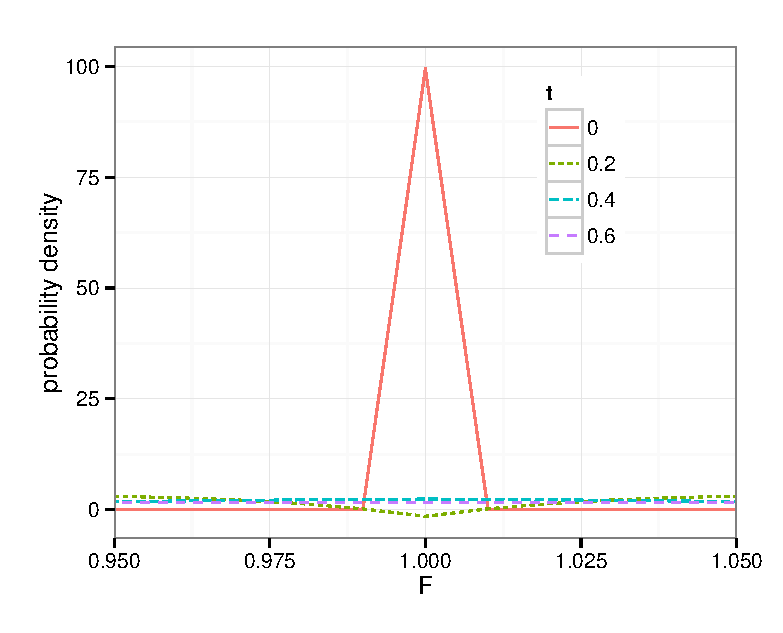
\includegraphics[width=7cm]{density_hagan_trbdf2_500_5_5.eps}}
%  \subfigure[TR-BDF3]{\label{fig:density_hagan_trbdf3_500_5_5}
%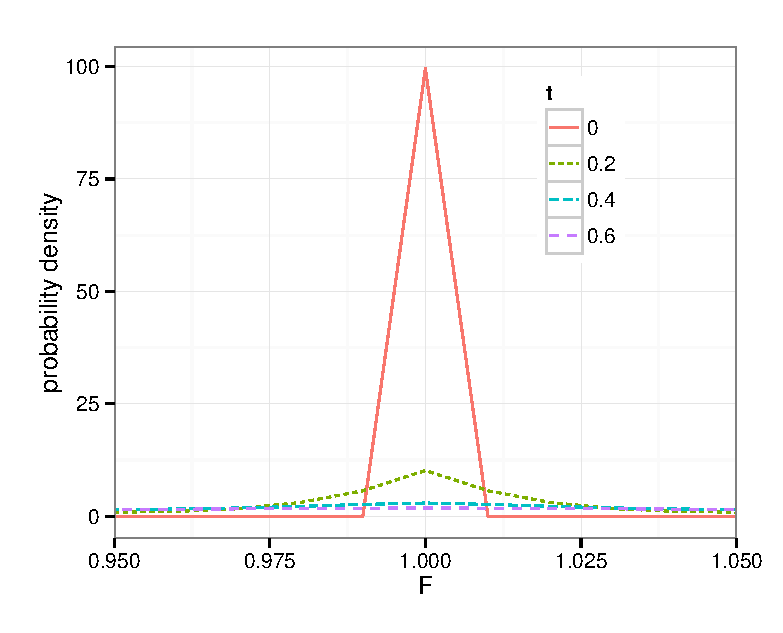
\includegraphics[width=7cm]{density_hagan_trbdf3_500_5.eps}}
%   \end{center}
%     \caption{Probability density in Hagan PDE using a total of 5 time-steps for the first 4 steps}
%\end{figure}
%
%\subsection{Convergence and Performance}

\end{document}
